\chapter[Tecnologias de Processo]{Tecnologias de Processo}
\label{chap:tecnologias}
	
	\section[Definição]{Definição}
	\label{sec:tecnologias_definicao}

		Qualquer operação utiliza algum tipo de tecnologia de processos, visando auxiliar o processo de produção a atender uma necessidade específica de seus clientes, podendo ser um simples processador de texto ou então uma grande fábrica automatizada, ou seja, tecnologia de processos são as máquinas, equipamentos e dispositivos que ajudam a gerar um produto final, seja ele um material, uma informação ou consumidores.\cite{slack}

		Frequentemente, as discussões acerca do Gerenciamento de Processos são marcadas pelo ponto chave "Tecnologia", de modo que temos uma prática focada nos processos e suportada por plataformas tecnológicas, ocorrendo assim uma integração entre os fatores negócios e tecnologias.\cite{lecom} 

		\begin{figure}[h]
			\centering
			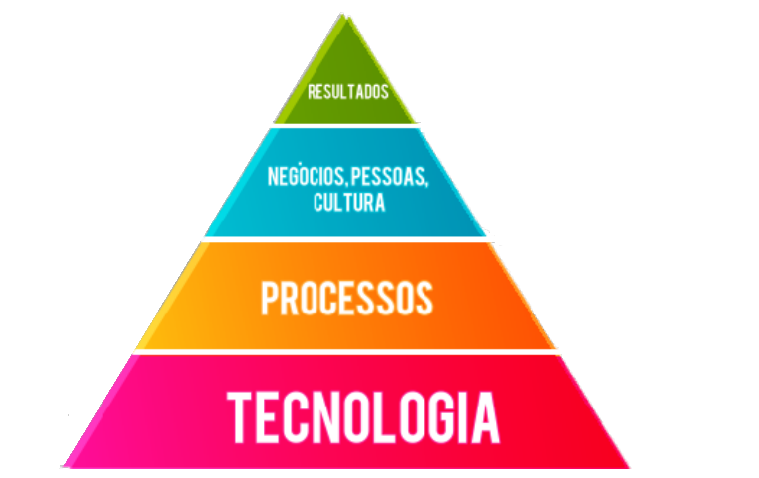
\includegraphics[scale=0.8]{tec1}
			\caption[O que suporta os resultados]{O que suporta os resultados.}
			\label{fig:tec1}
		\end{figure}

		Assim, a tecnologia auxiliará na hora de adequar os processos aos objetivos gerais da organização, gerando uma maior eficácia, eficiência e competitividade. Considerando ainda o nível de complexidade das tarefas e dinamicidade das mudanças, há uma necessidade de utilizar as tecnologias para a performance da organização, no quesito automatização de atividades e na integração de sistemas, indivíduos e ações. 

		\subsection[Tecnologia de processamento de Materiais]{Tecnologia de processamento de Materiais}
		\label{sec:tecnologias_definicao_materiais}

			Os avanços tecnológicos proporcionaram novas maneiras de processar materiais e, de acordo com \cite{slack}, podemos classificar em:

			\begin{itemize}
				\item{\textbf{Máquinas-ferramentas de controle numérico computadorizadas}: substituição da mão de obra humana por máquinas, visando uma maior produtividade e redução dos custos;}
				\item{\textbf{Robótica}: utilização de robôs em aplicações industriais como o empilhamento, soldagem, pintura, etc;}
				\item{\textbf{Veículos guiados automaticamente}: se resume no uso de veículos automatizados para transferir materiais fisicamente;}
				\item{\textbf{Sistemas flexíveis de manufatura}: junta tecnologia em um sistema único, ou seja, é um sistema capaz de desempenhar operações mecânicas, mover peças de uma estação para outra, controlar e coordenar as atividades;}
				\item{\textbf{Manufatura integrada por computador}: “[...] monitoramento baseado em computador e controle de todos os aspectos do processo de manufatura, baseado num banco de dados comum e comunicando por meio de alguma forma de rede de computadores”. \cite{dale}}
			\end{itemize}

		\subsection[Tecnologia de processamento de Informações]{Tecnologia de processamento de Informações}
		\label{sec:tecnologias_definicao_informacoes}
		
			\begin{itemize}
				\item{\textbf{Tecnologia de Processamento de Informação}: envolve qualquer dispositivo capaz de colher, manipular, armazenar e distribuir informação, como computadores;}
				\item{\textbf{Processamento de Informação Centralizada}: um único computador centralizado que armazenam as informações usando o processamento por lote (batch);}
				\item{\textbf{Processamento de Informações Descentralizadas}: processamento com distribuição ao longo de uma organização, sendo projetado para cada atividade específica.}
			\end{itemize}

		\subsection[Tecnologia de processamento de Consumidores]{Tecnologia de processamento de Consumidores}
		\label{sec:tecnologias_definicao_consumidores}

			Classifica aquelas interações entre o consumidor e a tecnologia, podendo ser direta, como um telefone, ou mediante intermediário, como reserva de um quarto de hotel. \cite{slack}

	\section[Gerenciamento de operações e tecnologia de processo]{Gerenciamento de operações e tecnologia de processo}
	\label{sec:tecnologias_Gerenciamento}
		
		Os responsáveis pelo gerenciamento de tecnologias de processo são os gerentes da produção e os mesmos precisam ter a capacidade de se relacionarem com a tecnologia em si sabendo as melhorias que podem ser causadas nas operações, integrar a tecnologia com a produção, monitorando o desempenho e atualizar ou substituir a tecnologia em caso de necessidade. 
		
		Não é necessário que os gerentes da produção sejam expert em alguma área específica, somente que saibam aplicar os conceitos de gestão e garantia de qualidade de modo que a performance de qualquer corporação seja impulsionado, utilizando os princípios apresentados pela norma NBR ISO 9000: \cite{lecom}

		\begin{itemize}
			\item{\textbf{Envolvimento dos indivíduos}: pelo fato de uma corporação ser composta por várias pessoas com um ou vários objetivos pré-determinados, o envolvimento dessas pessoas no processo de assimilação das políticas de qualidade é necessário para interagir e inserir as mesmas na organização, aproveitando as habilidades individuais;}
			\item{\textbf{Liderança}: os gerentes da produção ou líderes devem ser capazes de envolver as pessoas e entender a importância da gestão de qualidade e seus processos;}
			\item{\textbf{Foco no cliente}: "É recomendável que os requisitos organizacionais sejam motivados a atender e exceder as expectativas dos clientes.";}
			\item{\textbf{Relacionamento com fornecedores}: esse relacionamento deve possuir o benefício mútuo e a ampliação da capacidade de geração de valor agregado pela parceria como foco;}
			\item{\textbf{Melhoria Contínua}: a busca por uma constante melhoria no desempenho global deve ser considerado como um objetivo permanente. Um bom exemplo é o ciclo PDCA, que prevê o constante planejamento e re-planejamento de ações.}
		\end{itemize}

		\newpage
		\begin{figure}[h]
			\centering
			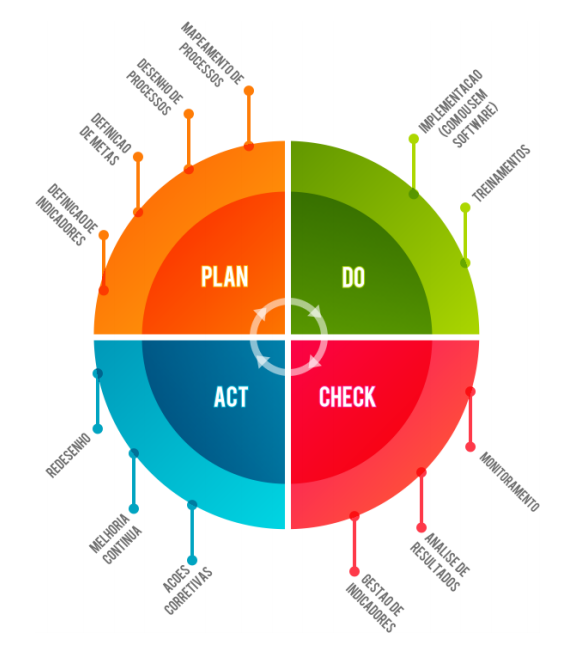
\includegraphics[scale=0.8]{tec2}
			\caption[Ciclo PDCA (Plan - Planejar, Do - Fazer, Check - Checar e Act - Agir) ]{Ciclo PDCA (\emph{Plan} - Planejar, \emph{Do} - Fazer, \emph{Check} - Checar e \emph{Act} - Agir).}
			\label{fig:tec2}
		\end{figure}

		Além desses princípios, os gerentes da produção devem ser capazes de lidar com os experts de tecnologia e realizar algumas perguntas para fazer um estudo acerca da tecnologia que será utilizada: 

		\begin{itemize}
			\item{O que a tecnologia é capaz de fazer? Qual a diferença entre ela e as outras tecnologias similares?}
			\item{Quais características particulares da tecnologia são usadas para realizar suas respectivas funções?}
			\item{Quais são os benefícios que a tecnologia pode oferecer?}
			\item{Quais são as limitações impostas pela tecnologia?}
		\end{itemize}

	\section[Aplicações]{Aplicações - 
\includegraphics{bobs2}}
	\label{sec:tecnologias_aplicacoes}

		A rede \textbf{Bob’s} adquire seus hambúrgueres, batata frita, sorvete, etc. por meio de seus fornecedores \cite{junior}, como foi especificado na seção logística, ainda assim é possível visualizar o impacto da tecnologia na gestão da rede.
	
		Uma pesquisa foi realizada na franquia \textbf{Bob’s} do \textbf{Taguatinga Shopping}, cujo questionário respondido se encontra na seção anexos. O consumidor realiza seu pedido no caixa, onde tem as seguintes opções de pagamento:

		\begin{itemize}
			\item{Dinheiro};
			\item{Cartão de Crédito};
			\item{Cartão de Débito};
			\item{Vale Ticket};
			\item{Vale Refeição};
		\end{itemize}

		Sendo que o esquema de pagamento diferente de uma franquia para outra, pois algumas são realizadas pelo computador e outras pelas máquinas de cartão e o pagamento de cada franquia é individualizado, somente o faturamento final que é centralizado e interligado com a matriz do \textbf{Bob’s}. Os preços são padronizados de acordo com a região, pois uma região que possui menos poder aquisitivo paga menos, portanto os preços da franquia do \textbf{Taguatinga Shopping} e do aeroporto não diferem, pois os dois se localizam no DF, que possui um custo de vida alto.

		A rede dispõe de um sistema de vendas, com a finalidade de monitorar os suprimentos de uma franquia ao dar os dados necessários ou então a própria franquia solicita os suprimentos via site. Todas as franquias se comunicam por meio de um \emph{extranet}, utilizando as novas campanhas do \textbf{Bob’s}.

		Para o atendimento do cliente, a franquia se dispõe de máquinas de cartão, máquinas de sorvete, saladeira, \emph{toaster}, fritadeira, chapa, estufa de carnes, máquinas de refrigerante e suco e geladeiras, mostrando que é indispensável o uso de tecnologia nas franquias. Os produtos como hambúrguer, batata frita, etc. são adquiridos por fornecedores homologados pelo \textbf{Bob’s} que sempre fazem os produtos no padrão definido pela rede e após o cliente realizar seu pedido, os sanduíches são montados nas próprias franquias conforme o pedido do cliente.

		\subsection[Tecnologia de Informação e Consumidor]{Tecnologia de Informação e Consumidor}
		\label{sec:tecnologias_tic}

			Na área de gestão de processos nas últimas décadas, houve um grande impacto de uma nova tecnologia, a internet, que se tornou uma nova aliada para qualquer tipo de negócio, visto que a empresa que utiliza a internet para divulgar seus produtos possui um alcance bem maior do que aquela empresa que não utiliza e possui seu alcance limitado. \cite{slack}

			A empresa de \emph{fast food} \textbf{Bob’s} possui um site, onde disponibiliza seu cardápio, juntamente com suas promoções, suas opções de \emph{delivery}, que pode ser realizado via telefone, computador e mobile por meio de um aplicativo, e um formulário para quem quer ser franqueado, mostrando que a internet é uma forte aliada para atrair clientes de várias faixas etárias. Além disso, a empresa possui certo alcance em redes sociais, permitindo solicitar um serviço de entrega utilizando a conta do \emph{facebook} e divulgando seus produtos por meio de uma página de \emph{facebook} que é atualizada semanalmente.
		
			Porém, a rede \textbf{Bob’s} não é a única que utiliza a internet, na imagem abaixo se encontra um gráfico que exibe o alcance das redes ao mostrar quais redes de \emph{fast food} são mais citadas em redes sociais. \cite{miti}

			\begin{figure}[h]
				\centering
				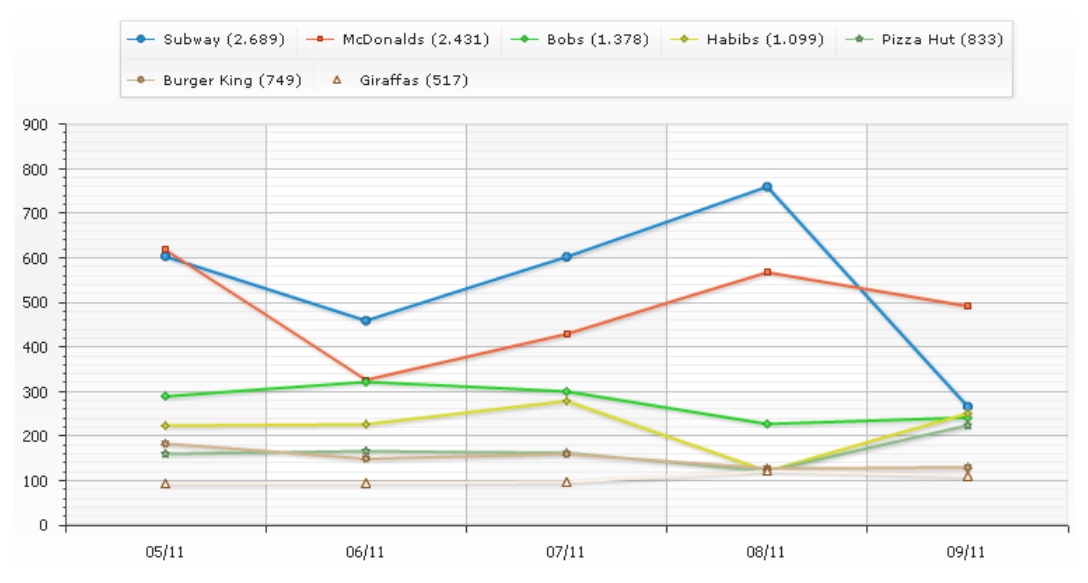
\includegraphics[scale=0.5]{tec3}
				\caption[Pesquisa acerca do alcance das redes de fast food via citações na internet em 2010, usando a ferramenta postX]{Pesquisa acerca do alcance das redes de \emph{fast food} via citações na internet em 2010, usando a ferramenta \textbf{postX}. \cite{miti}}
				\label{fig:tec3}
			\end{figure}

			Ao analisar a figura acima, é notável que \textbf{Bob’s} perde para outras redes de \emph{fast food}, mostrando que existia uma necessidade de reestruturar as táticas de marketing do \textbf{Bob’s} para que a empresa possa se diferenciar em um ambiente cada vez mais competitivo. 

		\subsection[Reestruturação]{Reestruturação}
		\label{sec:tecnologias_reestruturação}

			Apesar de perder para seus concorrentes nas redes sociais, a rede \textbf{Bob’s} conseguiu adotar medidas como a reduzir a verticalização e focar na qualidade do serviço e produto final ao vender suas fábricas de hambúrguer, batata frita, sorvete e refresco, permitindo assim a obtenção dos mesmos já prontos e um maior foco nas suas campanhas de marketing, treinamento de funcionários e desenvolvimento de novos produtos, alcançando uma expansão como mostrado na figura abaixo.

			\begin{figure}[h]
				\centering
				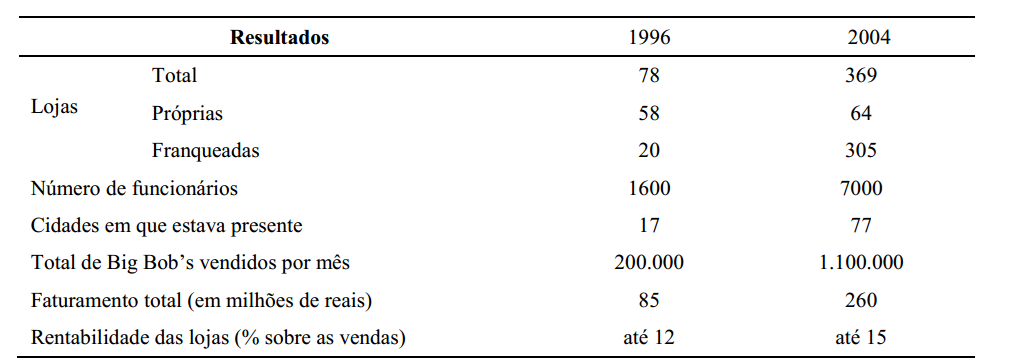
\includegraphics[scale=0.6]{tec4}
				\caption[Comparação dos resultados da rede Bob’s entre 1996 e 2004 ]{Comparação dos resultados da rede \textbf{Bob’s} entre 1996 e 2004. \cite{osman}}
				\label{fig:tec4}
			\end{figure}
